 %!TEX root = /Users/andy/Documents/Academics/Dissertation/thesis.tex

\chapter{Optogenetic manipulation of neural activity in freely moving \textit{Caenorhabditis elegans}}


\section{Introduction}
\lettrine{R}{easerchers in systems neuroscience} aim to understand how neural dynamics create behavior. Optogenetics has accelerated progress in this area by making it possible to stimulate or inhibit neurons that express light-activated proteins, for example, channelrhodopsin-2 (ChR2) and halorhodopsin (also known as Halo/NpHR), by illuminating them \citep{nagel_channelrhodopsin-2_2003, boyden_millisecond-timescale_2005, zhang_channelrhodopsin-2_2006, han_multiple-color_2007,szobota_remote_2007,zhang_multimodal_2007,chow_high-performance_2010}. 
The nematode \textit{C. elegans} is particularly amenable to optogenetics owing to its optical transparency, compact nervous system and ease of genetic manipulation \citep{nagel_light_2005, liewald_optogenetic_2008, guo_optical_2009,stirman_high-throughput_2010}.

The ability to deliver light to one cell with spatial selectivity is essential for targeted optogenetic perturbation in the many cases in \textit{C. elegans} in which genetic methods do not provide adequate specificity. In the worm motor circuit, for example, single neuron-specific promoters are not available to drive expression of light-activated proteins in only one or a few neurons of the ventral nerve cord (VNC).
Optogenetics has been applied to the mechanosensory circuit in \textit{C. elegans}, but only through simultaneous stimulation of all touch receptor neurons, because promoters specific to each neuron are unavailable \citep{nagel_channelrhodopsin-2_2003}. 
Researchers can use laser killing to study the contribution of single touch receptor neurons to overall behavior by removing neurons, but it is often preferable to work with intact circuits \citep{chalfie_neural_1985, wicks_dynamic_1996, kitamura_contribution_2001}.
Recently, a digital micromirror device (DMD) has been used to deliver light with high spatial selectivity in immobilized \textit{C. elegans} and immobilized \textit{Danio rerio} zebrafish \citep{wyart_optogenetic_2009}; each element of a DMD may be independently controlled to deliver light to a corresponding pixel of a microscope's field of view. 
In many cases, however, the normal operation of neural circuits can be studied only in freely behaving animals, requiring a more sophisticated instrument.

Here we describe an optogenetic illumination system that allows perturbations of neural activity with high spatial and temporal resolution in an unrestrained worm, enabling us to \emph{Co}ntrol \emph{L}ocomotion and \emph{Be}havior in \emph{R}eal \emph{T}ime (CoLBeRT) in\textit{C. elegans}. In the CoLBeRT system, a video camera follows a worm under dark-field illumination, and a motorized stage keeps the worm centered in the camera's field of view. Machine-vision algorithms estimate the coordinates of targeted cells within the worm body and generate an illumination pattern that is projected onto the worm by a DMD with laser light, and the cycle repeats itself for the next frame. Because the worm is a moving target, the faster an image can be captured and translated into DMD directives, the more accurately an individual cell can be targeted. The CoLBeRT system carries out all of these functions in \textasciitilde20 ms, providing a spatial resolution of \textasciitilde30 $\mu$m in optogenetic control for freely swimming\textit{C. elegans}. We analyzed the motor circuit and mechanosensory circuit of unrestrained worms, demonstrating the performance of the CoLBeRT system, a new tool that enhances the flexibility and power of optogenetic approaches in \textit{C. elegans}.

\section{Results}
\subsection{Experimental Setup}
To stimulate neurons using ChR2 or inhibit neurons using Halo/NpHR, we used a 473-nm or 532-nm wavelength diode-pumped solid state (DPSS) laser, respectively  (Fig.~\ref{fig:colbert1}a). Either laser was incident onto a DMD with 1,024 × 768 elements. Laser light was reflected onto the specimen only when an individual micromirror was turned to the 'on' position. We illuminated the specimen under dark-field illumination by red light to avoid exciting ChR2 or Halo/NpHR. Filter cubes reflected the wavelengths for optogenetic illumination from the DMD onto the sample, while passing longer wavelengths for dark-field illumination to a camera. A motorized stage kept the specimen in the field of view.



\begin{FPfigure} 
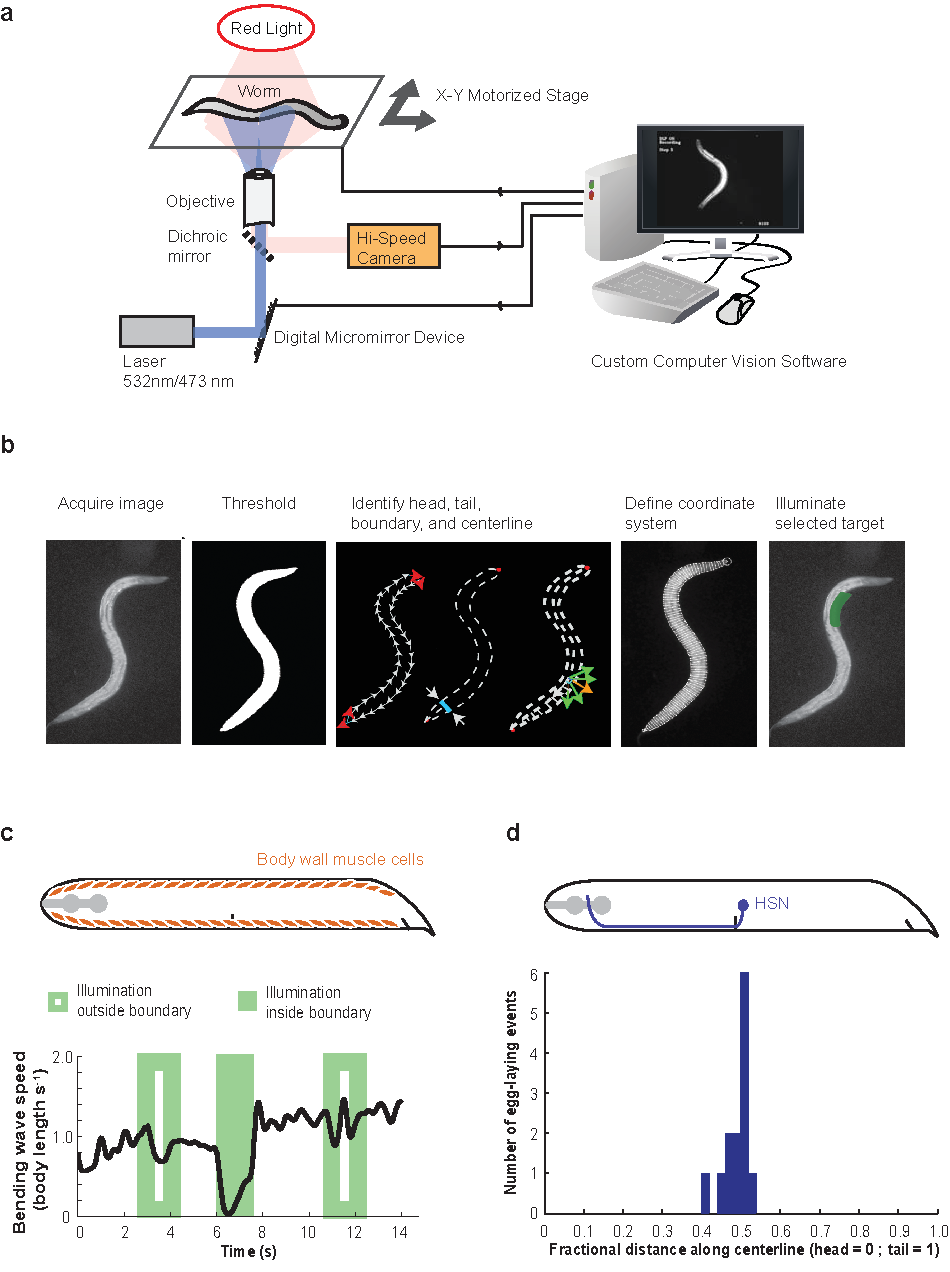
\includegraphics[width=\textwidth]{figures/colbert1}
\caption[CoLBeRT system apparatus and methodology]{ \textbf{(a)} An individual worm swims or crawls on a motorized stage under red dark-field illumination. A high-speed camera images the worm. Custom software instructs a DMD to reflect laser light onto targeted cells. \textbf{(b)} Images are acquired and processed at ~50 FPS. Each 1,024 × 768 pixel image is thresholded and the worm boundary is found. Head and tail are located as maxima of boundary curvature (red arrows). Centerline is calculated from the midpoint of line segments connecting dorsal and ventral boundaries (blue bar) and is resampled to contain 100 equally spaced points. The worm is partitioned into segments by finding vectors (green arrows) from centerline to boundary, and selecting one that is most perpendicular to the centerline (orange arrow). Targets defined in worm coordinates are transformed into image coordinates and sent to the DMD for illumination (green bar). \textbf{(c)} Schematic of body-wall muscles. Anterior, to left; dorsal, to top. Bending wave speed of swimming worm expressing Halo/NpHR in its body-wall muscles subjected to green light (10 mW mm$^{-2}$) outside or inside the worm boundary (n = 5 worms, representative trace). \textbf{(d)} Schematic of HSN. A swimming worm expressing ChR2 in HSN was subjected to blue light (5 mW mm$^{-2}$). Histogram, position at which egg-laying occurred when a narrow stripe of light was slowly scanned along the worm's centerline (n = 13 worms). Once an egg was laid, the worm was discarded. \label{fig:colbert1}}
\end{FPfigure}

To accelerate real-time image analysis of worm posture, we developed the MindControl software package using the open-source OpenCV computer vision library\citep{bradski_opencv_2000}. With the graphical user interface (GUI), the user can dynamically target specific regions of freely moving worms. The MindControl software and documentation are available at \href{http://github.com/samuellab/mindcontrol}{http://github.com/samuellab/mindcontrol}.


The MindControl software carries out a sequence of image analysis operations on each frame received from the camera (Fig.~\ref{fig:colbert1}b). An image is captured by the computer, filtered and thresholded. Next, the boundary of the worm is calculated, and head and tail are identified as local maxima of boundary curvature (the head is blunt and the tail is sharp). The worm centerline is calculated and the body is divided into 100 evenly spaced segments. These segments define a worm coordinate system invariant to worm posture or orientation, within which the user may define target positions. The software maps the position of targets onto the coordinates of the real image and finally sends the appropriate pattern to the DMD for illumination.

For our current system, the total latency between image acquisition and DMD illumination is 20~ms: image exposure, 2~ms; data transfer to computer, 3~ms; image analysis, 10~ms; and data transfer to DMD, 5~ms. Given the size and speed of a swimming worm at 10× magnification, our system working at \textasciitilde50 frames per second (FPS) delivers optogenetic illumination with a spatial resolution of \textasciitilde30~$\mu$m, not far from the spatial resolution limit imposed by the pixel density of the DMD (\textasciitilde5~$\mu$m at 10× magnification).

\subsection{Spatial resolution of the illumination system}
First, we confirmed that illumination is restricted to the targeted area. We examined a transgenic worm expressing \textit{Halo/NpHR::CFP} in all body-wall muscles. Whole-animal illumination of transgenic P\textit{myo-$3$::Halo/NpHR} worms causes all muscles to relax \citep{zhang_multimodal_2007}. We placed individual swimming worms in the CoLBeRT system and used green light (532 nm, 10 mW mm$^{-2}$) to alternately illuminate the entire region outside and inside the worm boundary (Fig.~\ref{fig:colbert1}b and Supplementary Video 1). Illuminating the entire region outside the worm boundary had no effect as bending waves propagated from head to tail at normal speed. Illuminating the entire region inside the worm boundary, however, arrested locomotion as the body relaxed and the speed of bending waves dropped to zero.

To quantify the spatial resolution of the CoLBeRT system, we measured its targeting accuracy in evoking egg-laying events by stimulating the HSN motor neurons. We used transgenic worms expressing ChR2 under the \textit{egl-6} promoter, which drives expression in the bilaterally symmetric HSN neurons (HSNL and HSNR) as well as glia-like cells in the worm's head  \citep{ringstad_fmrfamide_2008}. Optogenetic stimulation of the HSN neurons, which innervate the vulval musculature, evokes egg-laying behavior (L. Emtage and N. Ringstad, personal communication).

The two HSN neurons lie on top of one another when the worm is viewed laterally, so our system targets both neurons. We projected a thin stripe of blue light (473 nm, 5 mW mm$^{-2}$) on the body of swimming P\textit{egl-6d::ChR2} transgenic worms. The long axis of the stripe was orthogonal to the worm centerline and spanned its diameter. The stripe width corresponded to 2\% of the anterior-posterior length of the worm centerline (that is, \textasciitilde20 $\mu$m of the \textasciitilde1-mm-long young adult worm). We used narrow stripes so that our illumination would be less probable to stimulate HSN when illuminating its process. We slowly moved the illumination stripe along the centerline of swimming worms while recording egg-laying events. Of 14 worms studied, we observed 13 egg-laying events, eight in which the stripe started at the head and five in which the stripe started at the tail. Egg-laying frequency sharply peaked when the center of the stripe coincided with the centerline coordinate of the HSN cell bodies, or 49.6\% of the total distance from the anterior to the posterior of the body with 3.2\% s.d. (Fig.~\ref{fig:colbert1}d and Supplementary Video 2). The width of this distribution suggests that the CoLBeRT system provides at least \textasciitilde30 $\mu$m of spatial resolution.
